\resetfigpath{Cases}


%%%{INTRODUCTION to this CHAPTER}%%%
In this section two applications using the proposed driver behavior model are explored. The first application investigates the relations  between driver behaviors and traffic accidents. The proposed method show the potential to identify the rationales behind a crash and provide a probability that similar crashes will repeat. The second application identifies driver's individual parameters to better predict the behaviors using the proposed method. 


\subsection{On Crash Investigations}
\label{subsec:CrashSim}

Although reasons behind each traffic accident vary with a broad possibilities from weather conditions to  infrastructure design, traffic accidents happen more frequently in some regions and intersections. In Section \ref{sec:Method}, the TFA distribution is defined as the probability density function of the driver taking actions (e.g. braking) under different TTC. The closer the current TTC to the mean TFA of the driver, the more likely the driver will brake at this TTC. As a consequence, in the \textbf{normal} cases (where vehicles passed or yield without collisions), drivers brake at TTCs within the TFA distribution to avoid potential collisions, and most of the TTCs that drivers brake at are those being closer to the mean value of the TFA distribution (those with higher likelihood). A greater TTC value implies more  conservative driving patterns and a smaller TTC value indicates more aggressive driving behaviors. 

\begin{figure}[htbp!]
    \centering
    \subfloat[The velocities versus POYs of a normal case where no collision happened.]
    {
    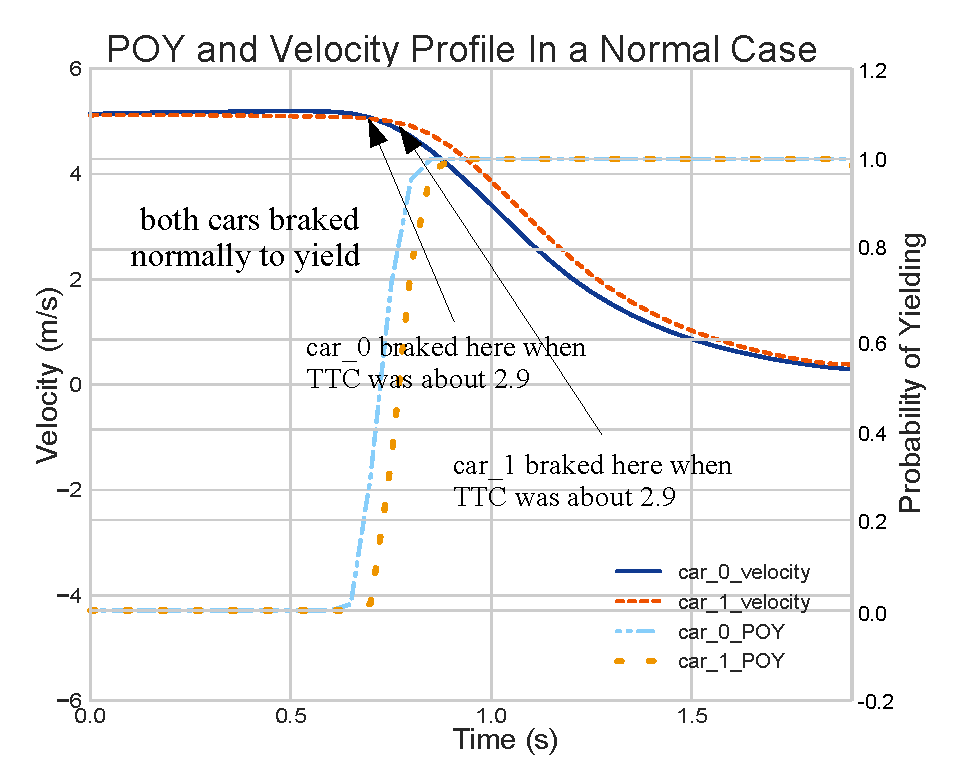
\includegraphics[width=0.48\textwidth]{case_normal_vel.pdf}
    \label{fig:normal015}
    }\hfill
    \subfloat[TFA distributions of Participant 1, 2 and average of a normal case where no collision happened.]
    {
    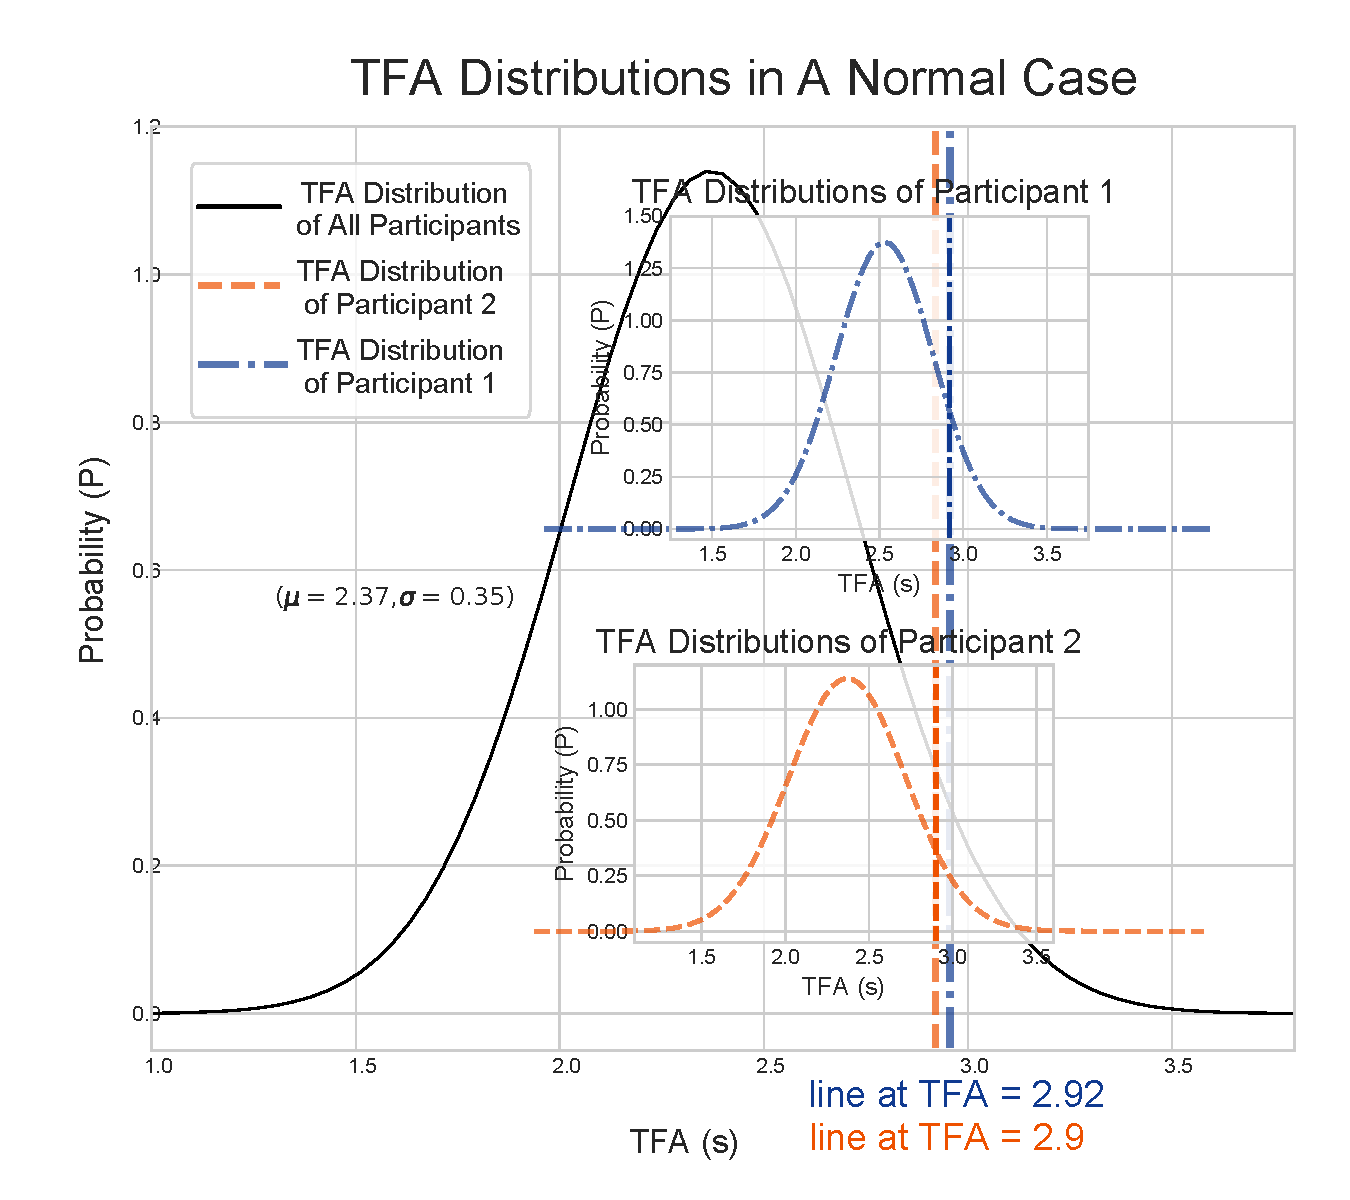
\includegraphics[width=0.48\textwidth]{case_normal_distribution.pdf}
    \label{fig:TFAs_normal015}
    }\hfill
    \caption{Velocity profile, POY and TFA distributions of participants of a case in real world where no collision happened.}
\label{fig:case_normal} 
\end{figure}


Consider the TFA distributions of a normal case with no accidents as shown in Fig.~\ref{fig:normal015} and Fig.~\ref{fig:TFAs_normal015}. The velocities and displacements of both vehicles are shown in Fig.~\ref{fig:normal015}, where both vehicles yielded at around $t=0.7$ sec to avoid potential collisions. When looking closer at the point of braking of both vehicle, the situation at this moment could be described using the concepts of TFA distributions as shown in Fig.~\ref{fig:TFAs_normal015}. The TFA distribution in black solid line is the average TFA distribution of all people, as illustrated and identified in Section \ref{subsec:TFADistribution}. Two vertical dash lines (all-dash and dash-dot) indicate the TTCs of Car\_0 (the driver is Participant 1) and Car\_1 (the driver is Participant 2) at braking, which are 2.92 and 2.90 respectively (brakes were applied at around 0.7 sec in Fig.~\ref{fig:normal015}). Sub-figures with dashed TFA distributions are the TFA distributions of Participant 1 and 2 (drivers of Car\_0 and Car\_1 respectively). In this case, both drivers brake at the TTC with relatively high likelihood (around 0.4) in the average TFA distribution.

Let us look at a case where collision happened in Fig.~\ref{fig:accident004} and Fig.~\ref{fig:TFAs_accident004}. The velocities and displacements of both vehicles are shown in Fig.~\ref{fig:accident004}, two vehicles eventually collided with each other at $t=3.6$ secs. 

\begin{figure}[htbp!]
    \centering
    \subfloat[The velocities versus POYs of a normal case where no collision happened.]
    {
    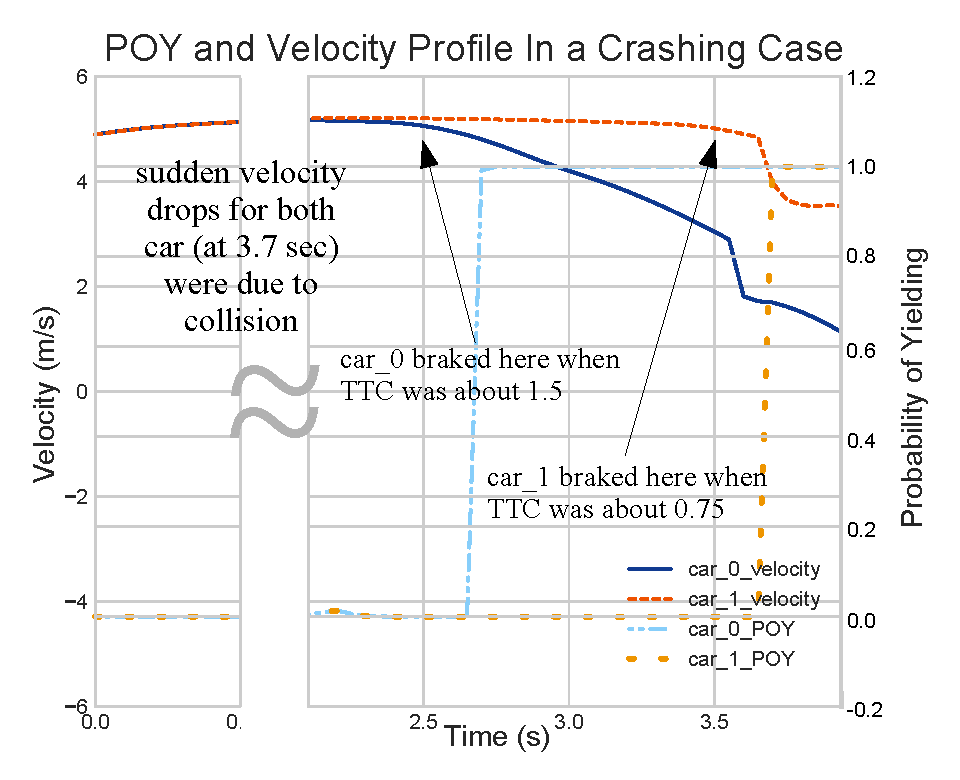
\includegraphics[width=0.48\textwidth]{case_accident_vel.pdf}
    \label{fig:accident004}
    }\hfill
    \subfloat[TFA distributions of Participant 1, 2 and average of a normal case where a collision did happen.]
    {
    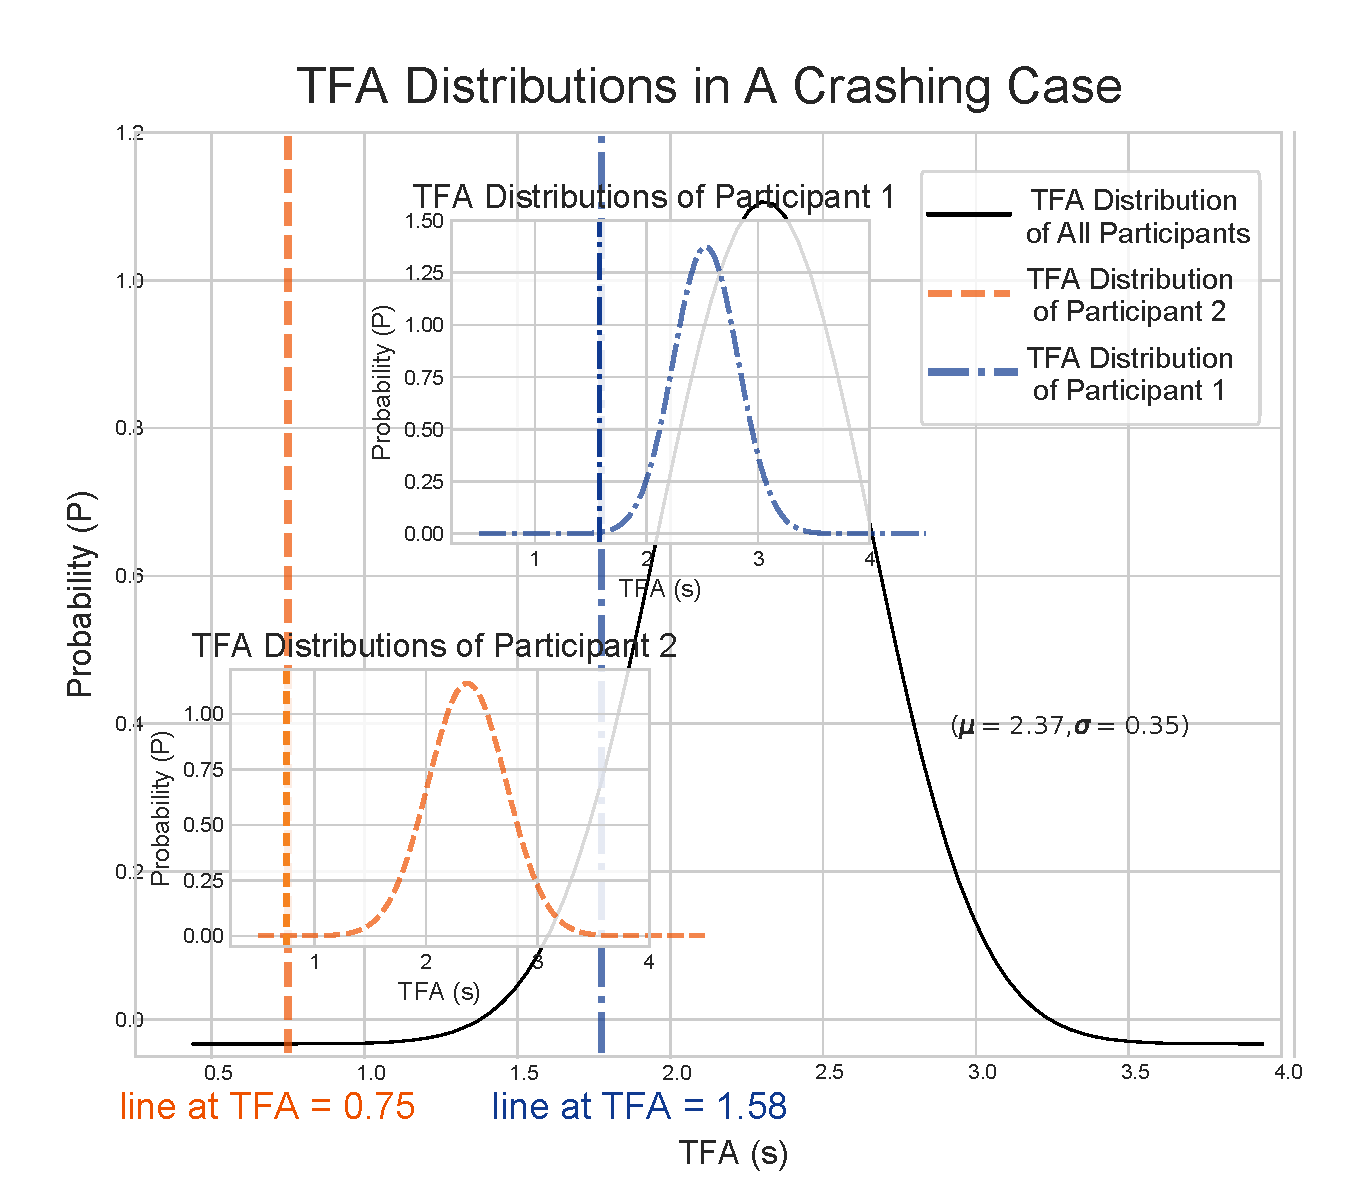
\includegraphics[width=0.48\textwidth]{case_accident_distribution.pdf}
    \label{fig:TFAs_accident004}
    }\hfill
    \caption{Velocity profile, POY and TFA distributions of participants of a case in real world where collision did happen.}
\label{fig:case_accident} 
\end{figure}


In Fig.~\ref{fig:accident004}, driver of Car\_0 (i.e. Participant 1) believed that the other driver would yield to him, while driver of Car\_1 (i.e. Participant 2) did not even noticed Car\_0 (possibly due to the lack of concentration and obstructions of his view), so they both approached to the intersection with max speed. At around 2.5 sec, Participant 1 finally braked because he realized that the collision was going to happen, and Participant 2 braked at aroundd 3.5 sec, right before the collision. Still, the late braking did not prevent the collision from happening at around 3.6 sec. The TFA distributions of this scenario, shown in Fig.~\ref{fig:TFAs_accident004}, indicates that the TTCs at the moment of braking for two drivers, 0.75 for Participant 2 and 1.50 for Participant 1 respectively, have low likelihoods, both below 0.1, to brake. Both drivers' low TTCs also represent aggressive behaviors (brake at shorter distances under the same speed).

Comparing the crashing case (Fig.~\ref{fig:TFAs_accident004}) to the normal case where no collision happened (Fig.~\ref{fig:TFAs_normal015}), we can readily see that the behaviors of drivers in the crash case tend to be more aggressive (the TFAs of drivers are very low, i.e. they brake at very low TTCs) and they are also less likely to happen (very low likelihood). This finding not only shows that the concept of the proposed model is effective, but also provides a different way to examine the likelihood of accidents happening under some particular behaviors. For example, when drivers at certain crossroads are found to have braking TTCs on the far-left side of the average TFA distribution, the possibilities of accidents in these crossroads are higher and similar scenarios are less likely to happen in a normal braking process (the TFA distribution).


%%%%%%%%%%%%%%%%%%%%%%%%%%%%%%%%%%%%%%%%%%%%%%%%%%%%%%%%%%%%%%%%%%%%%%%%%%%%%%%%%%%%%%%%%%%%%%%%%%%%%%%%%%%%%%%%%%%%%%%%%%%%%%%%%%%%%%

\subsection{On Driver Behavior Parameters Assessments}
\label{subsec:CharaParam}

People have their preferred ways of driving, some are aggressive, some are conservative, and many more average drivers among us. The parameters $R_{\mathrm{min}}$ and $a_{\mathrm{dec}}$ in TFA distributions reflect these driver behaviors: aggressive drivers tend to brake as late as possible, resulting a small $R_{\mathrm{min}}$. Similarly, drivers who drive offensively have higher $a_{\mathrm{dec}}$ values. Identifying an individual driver's parameters enables more accurate POY predictions, which will give rise to better classification rate $R_{\mathrm{CA}}$. Let us use the term 'general parameters' to reflect the parameters for an average driver and 'individual parameters' for a specific driver we would like to study.  In this section, the classification rate $R_{\mathrm{CA}}$ as defined in Eq.(\ref{eq:CARate}) will be used to determine if the individual parameters of a driver is correctly identified. 


% \begin{figure}[htbp!]
% \begin{center}
% \makebox[0pt]{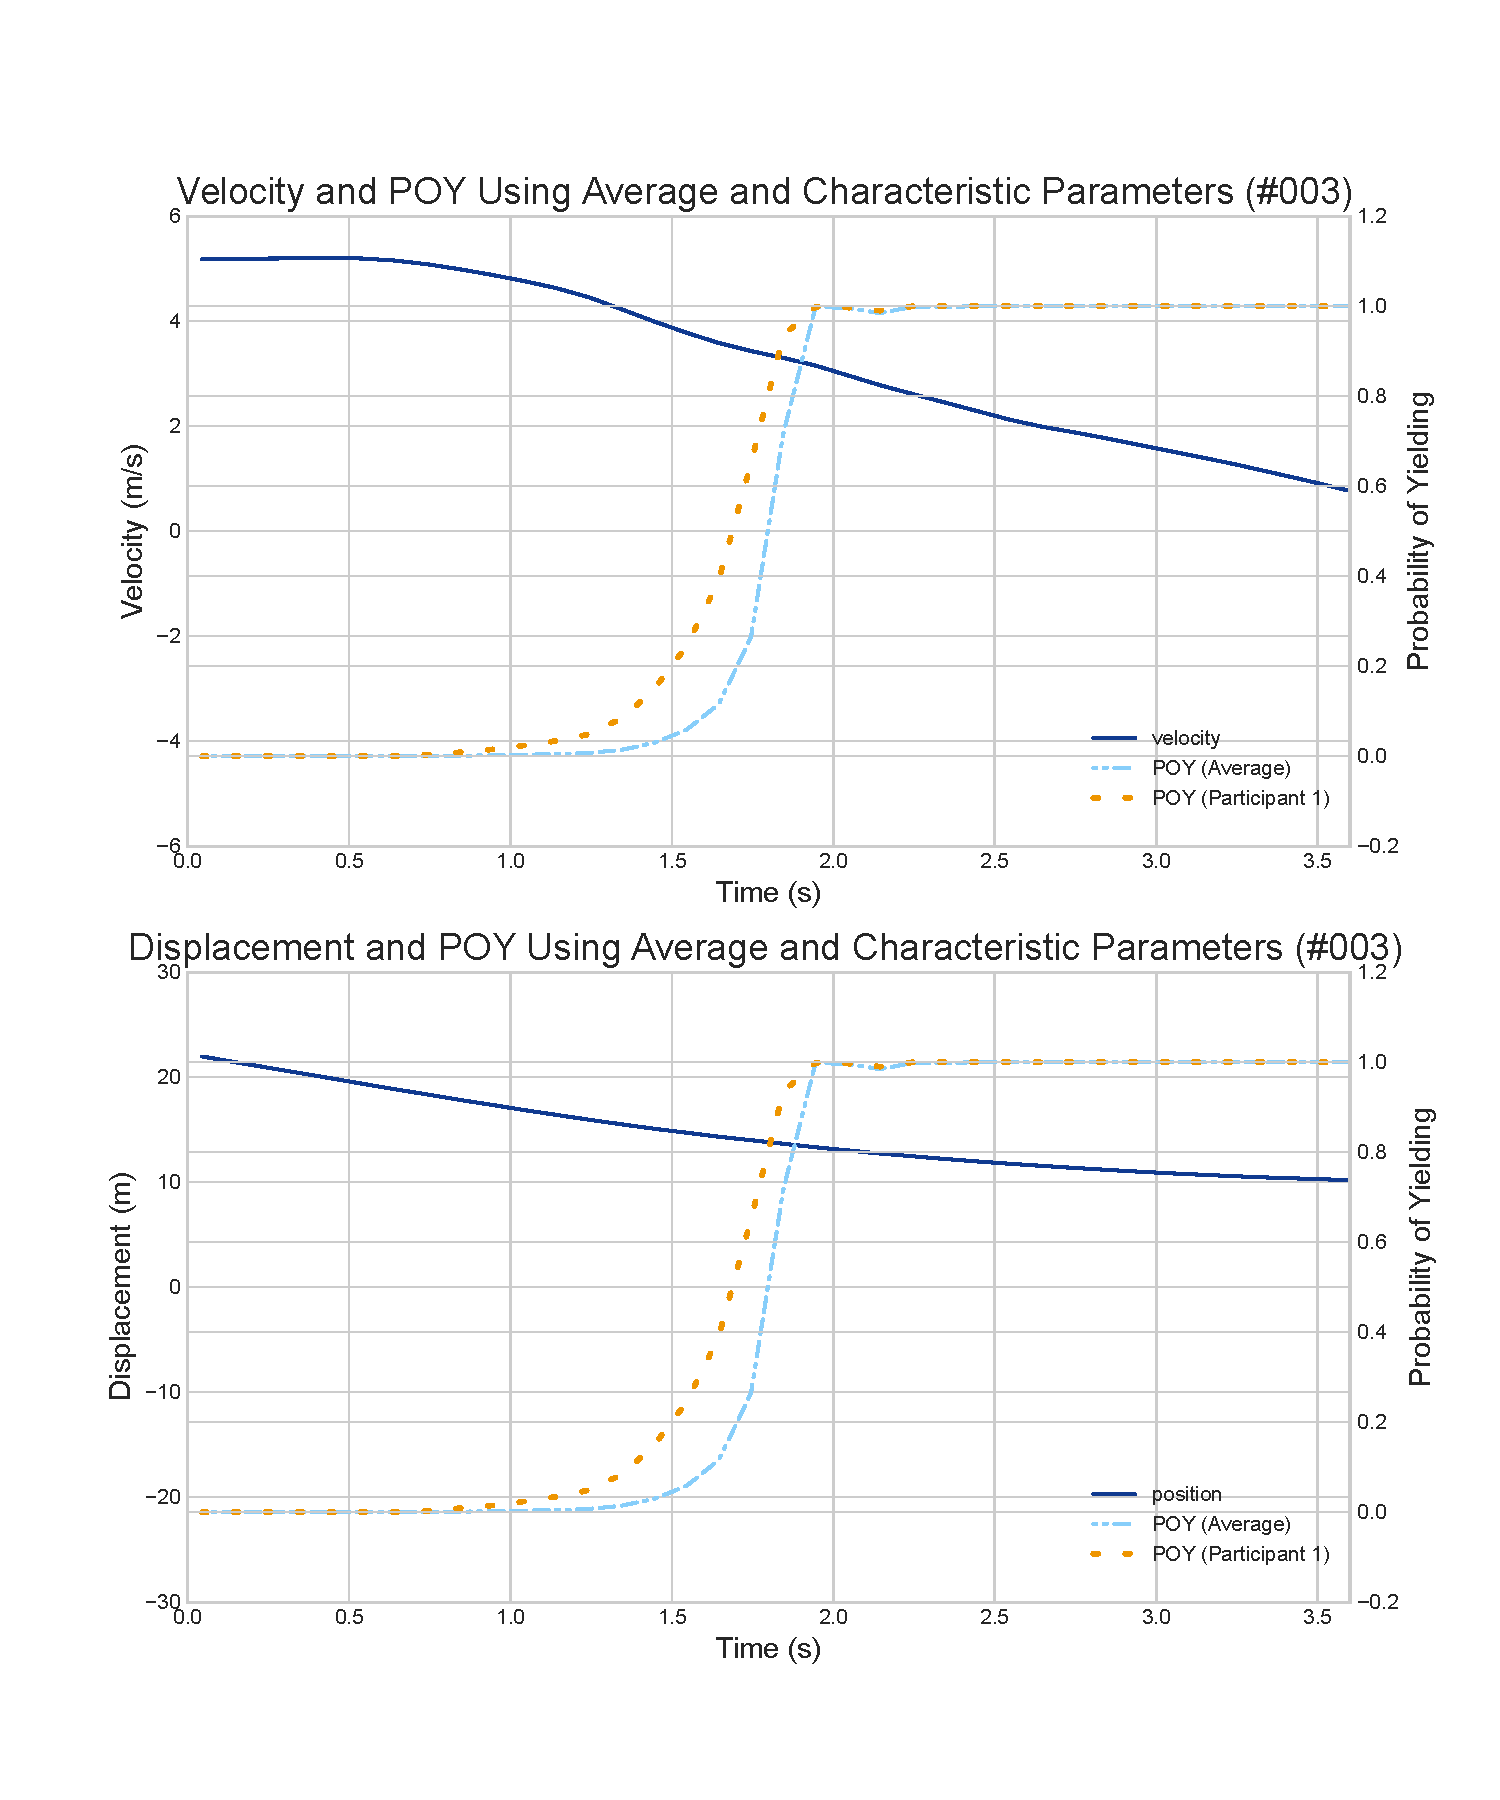
\includegraphics[width=0.85\paperwidth]{compare_trial_003.pdf}}
% \end{center}
% \caption{Trial \#003 with POY using general parameters and that of Participant 1.}
% \label{fig:trial003params} 
% \end{figure}

% \begin{figure}[htbp!]
% \begin{center}
% \makebox[0pt]{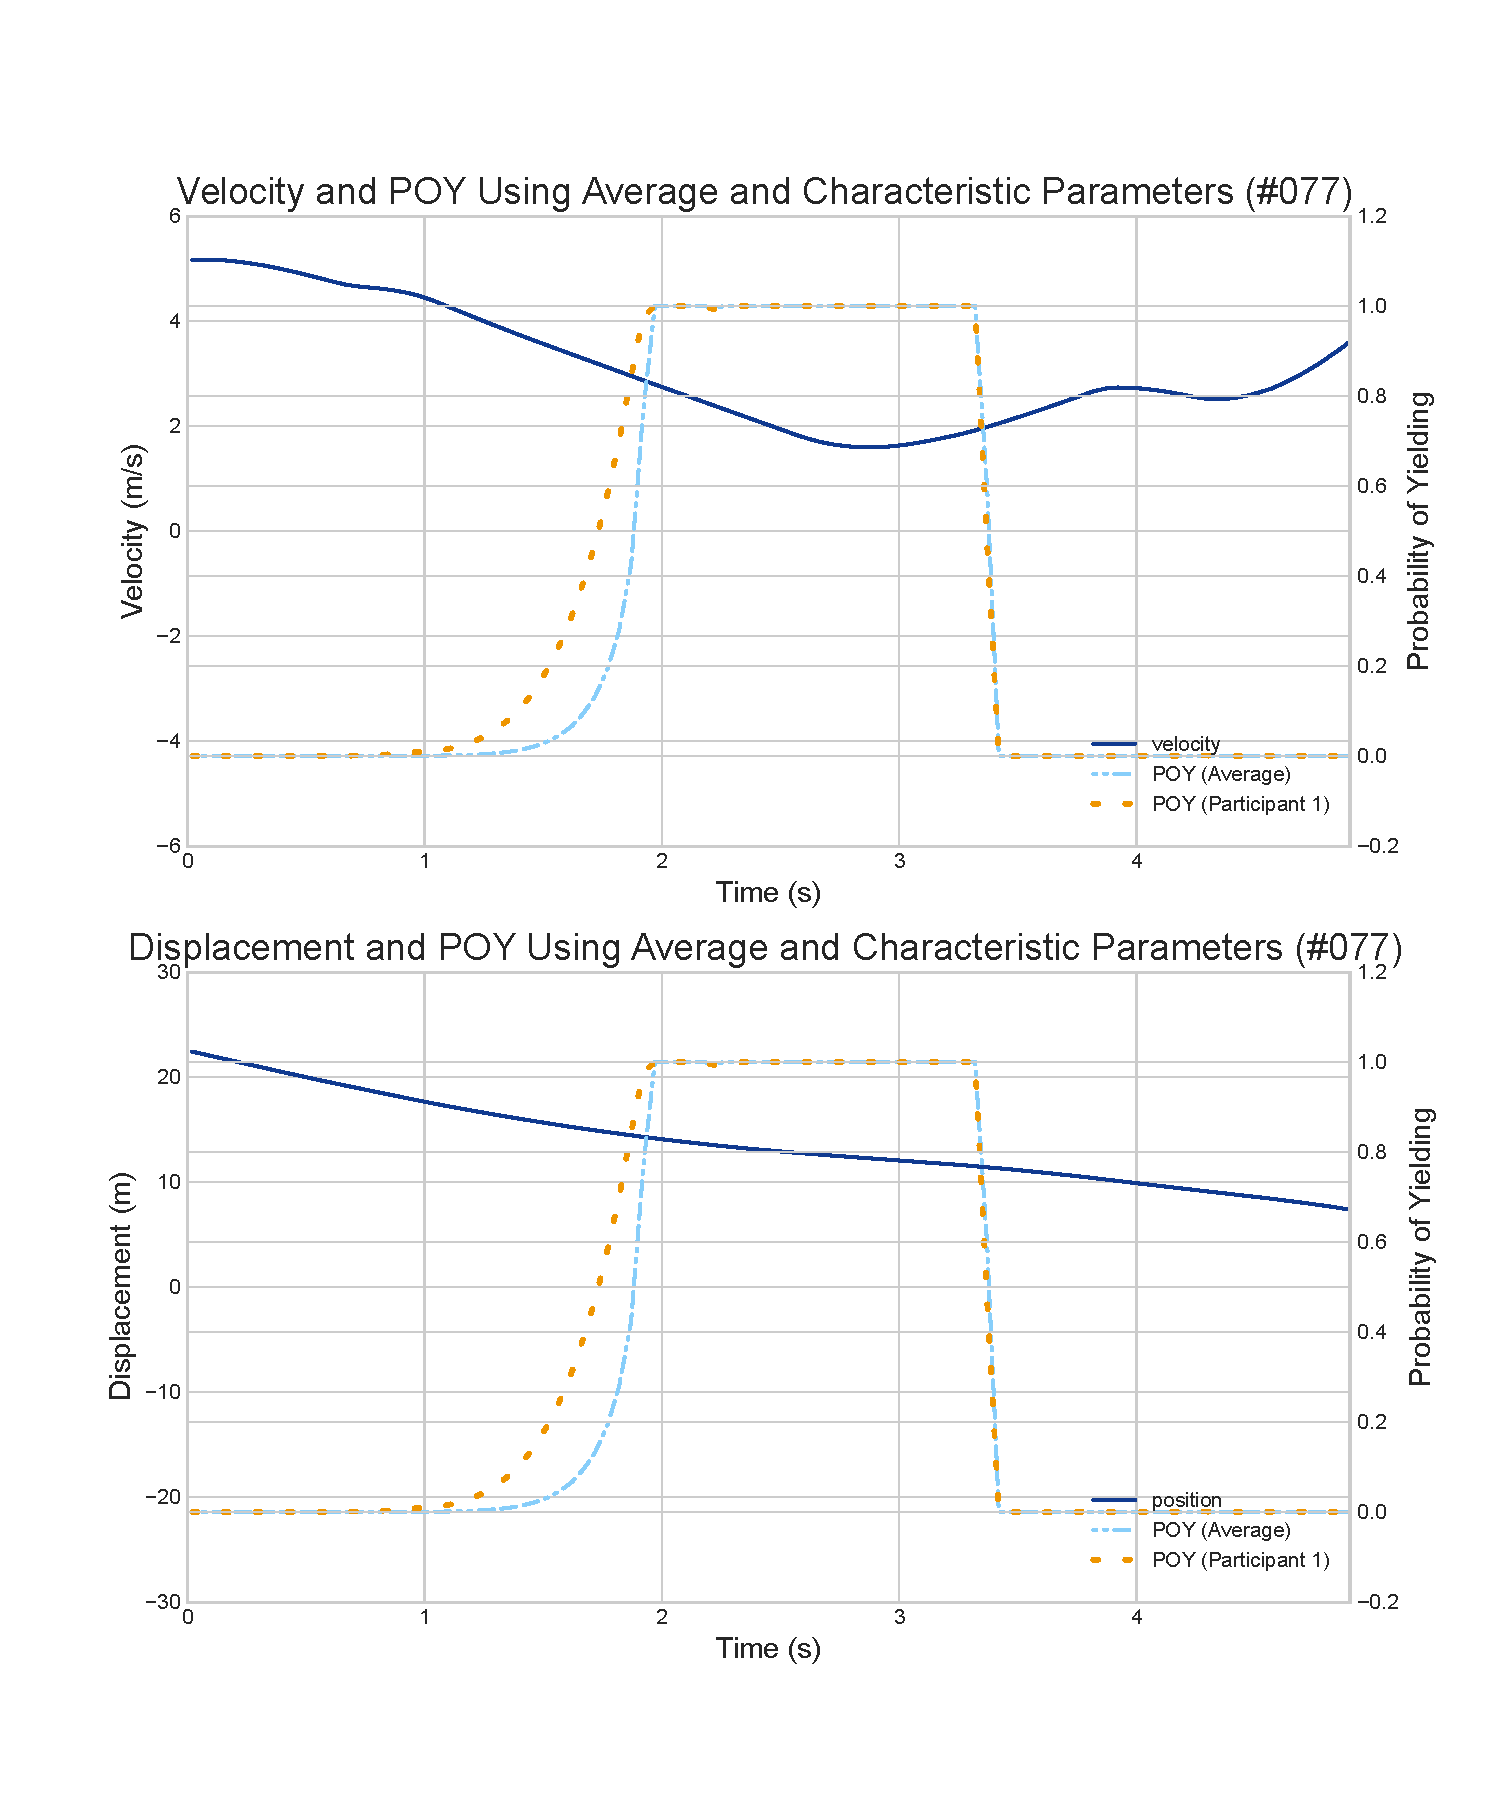
\includegraphics[width=0.85\paperwidth]{compare_trial_077.pdf}}
% \end{center}
% \caption{Trial \#077 with POY using average parameters and that of Participant 1.}
% \label{fig:trial077params} 
% \end{figure}

Fig.~\ref{fig:CAR_twoParticipants} shows two $R_{\mathrm{CA}}$ curves generated from a series of two-car crossroad interactions. Similar to Fig.~\ref{fig:CARPOY}, The $x$-axis is the reversed time before the end of the incident. A trend line of $R_{\mathrm{CA}}$ curves between $\mathrm{T}_{\mathrm{minus}} = 0$ and $\mathrm{T}_{\mathrm{minus}} = 1$ is plotted, showing a reasonable $R_{\mathrm{CA}}$ curve, where $R_{\mathrm{CA}}$ should be higher toward the end of the incident ($\mathrm{T}_{\mathrm{minus}} = 0$). The solid line represents the $R_{\mathrm{CA}}$ curve of a driver throughout the interactions, where individual parameters are used in the POY model. The dash-dot line is the $R_{\mathrm{CA}}$ curve of the same driver with a different set of parameter values. We can see that using the individual parameters could effectively narrow down the TFA of the driver to within the more precise TFA distribution.

%Providing general parameters into Eqn.~\ref{eq:TFA_est} yields a rough estimates of the TFA of the driver at the moment (considering velocity, displacement to the node and so on). 

\begin{figure}[htbp!]
\begin{center}
\makebox[0pt]{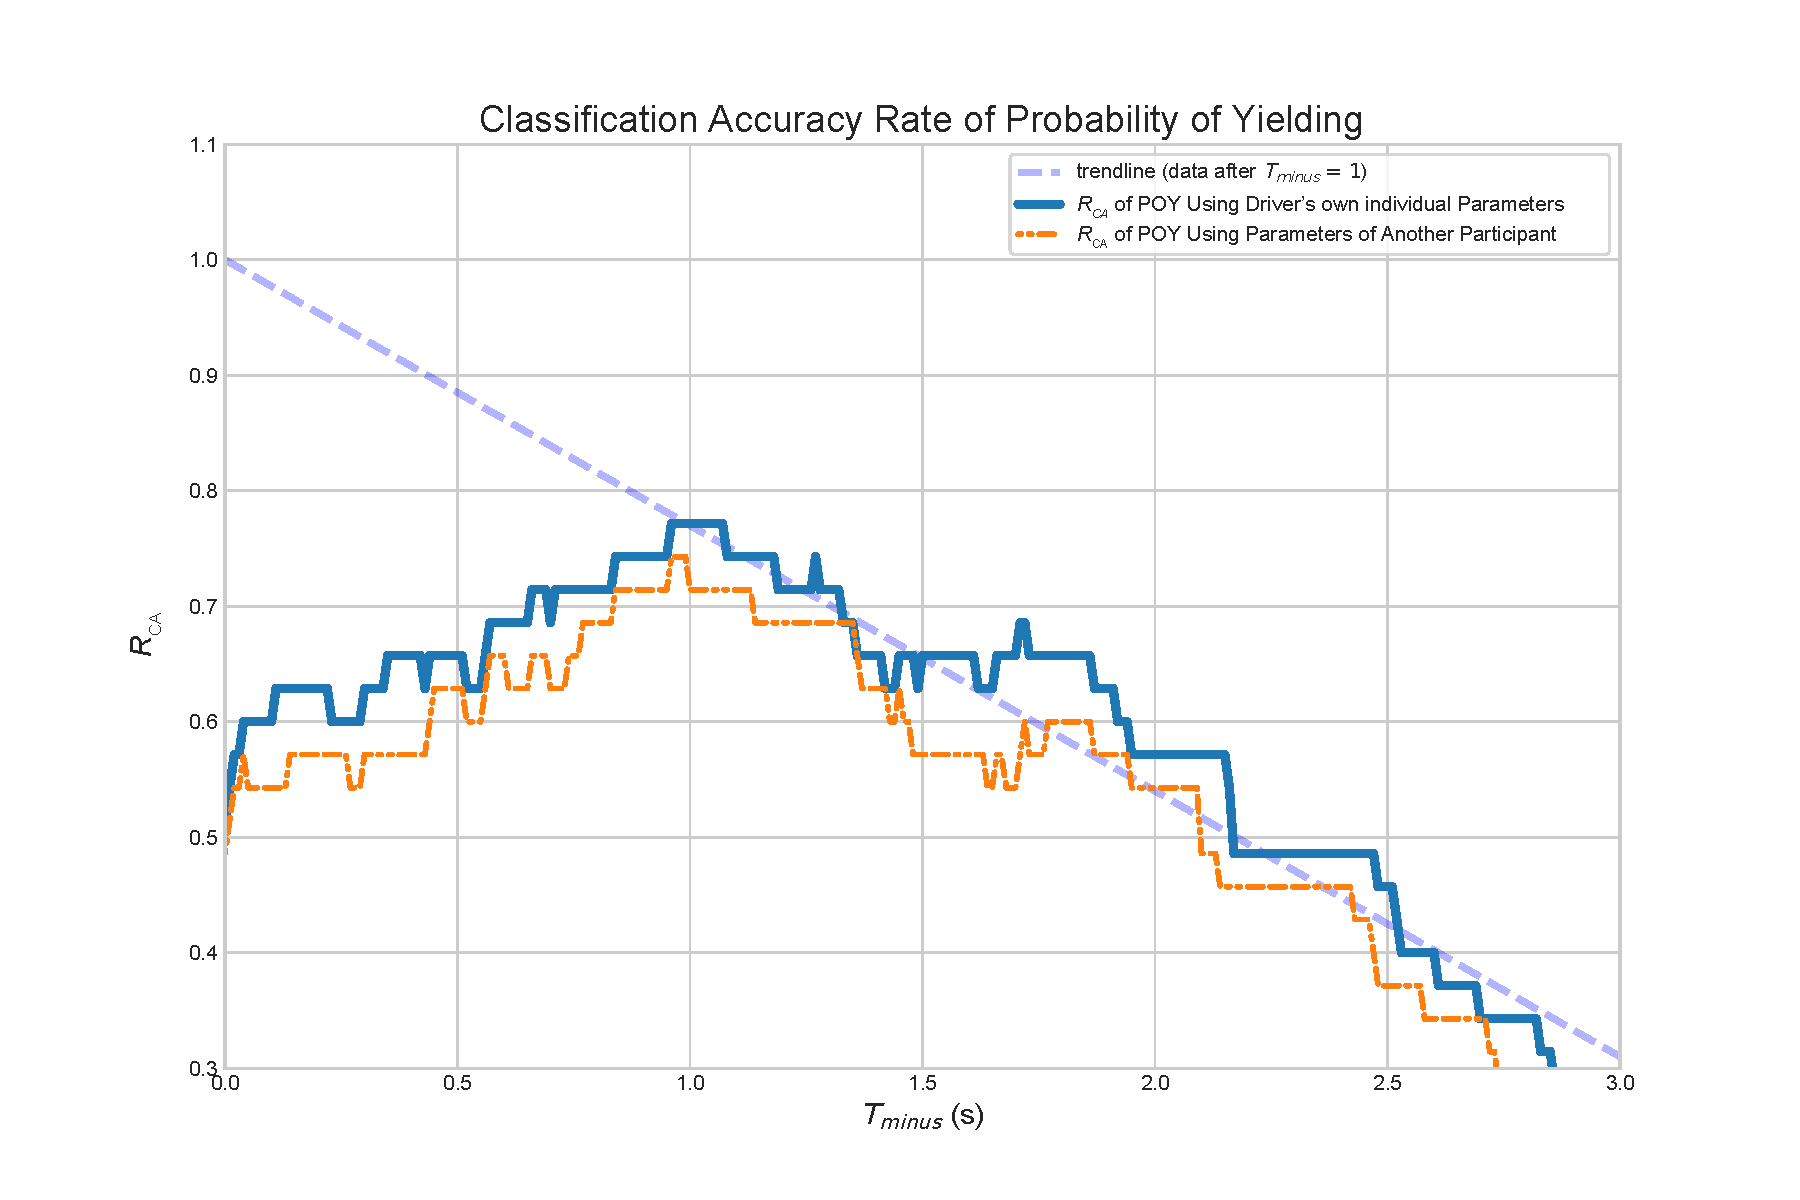
\includegraphics[width=0.64\paperwidth]{CARPOY_twoParticipants.pdf}}
\end{center}
\caption{$R_{\mathrm{CA}}$ curves of POY using driver's own individual parameters and the parameters set of another participant.}
\label{fig:CAR_twoParticipants} 
\end{figure}


\begin{table}[htbp]
\caption{Table for individual and general parameters.}
\begin{center}
\label{table:character_average}
\begin{tabular}{l l c c c}
% & & \\ % put some space after the caption
\hline
\textbf{Parameters} &  &\textbf{General} &\textbf{Participant 1} &\textbf{Participant 2} \\
\hline
Safe Margin Coefficient (${C1}_{\mathrm{Rmin}}$)     & & 0.295 & 0.166 & 0.390 \\
Safe Margin Constant (${C2}_{\mathrm{Rmin}}$)        & & 5.47 & 6.19 & 5.54  \\
Deceleration Coefficient (${C1}_{\mathrm{adec}}$)    & & 0.458 & 0.465 & 0.710 \\
Deceleration Constant (${C2}_{\mathrm{adec}}$)       & & 0.877 & 0.377 & 0.813 \\
% Standard Diviation Parameter ($\gamma$)     & & 0.148 & 0.115 & 0.102 \\
\hline
\end{tabular}
\end{center}
\end{table}



We have shown that accurate parameters provide a better (higher) $R_{\mathrm{CA}}$ curve. Optimizing $R_{\mathrm{CA}}$ using Eq.\ref{eq:optimize_POY} could lead to the true individual parameters. The objective function in Eqn.~\ref{eq:optimize_POY} indicating our goal to maximize the total area underneath the $R_{\mathrm{CA}}$ curve, where the $w$ is the parameters set. The constants $M$ and $N_j$ stand for the number of the trials in the collected data and the number of time steps in each trial with the resolution of 0.01 sec. The constraints in Eqn.~\ref{eq:optimize_POY} are defined by the minimum and maximum values of $R_{\mathrm{min}}$ and $a_{\mathrm{dec}}$ in the simulated environment, which are the distances between two cars and acceleration capabilities, respectively. In this study, we use \ac*{SA}  due to the non-smooth and time-consuming properties of the objective function. 

% Since our goal is to : 

% \begin{equation}
%     \mathrm{maximize} ~~ \big\{ \text{area under $R_{\mathrm{CA}}$ curves} \big\} 
% \label{eq:text_obj_function}    
% \end{equation}


    \begin{mini}|l|
	  {w}{\frac{1}{M}~\sum_{j=1}^{M}\sum_{i=1}^{N_j}{- f( { \mathrm{POY}}_{j}(t_i, w))}}{}{}
	  \addConstraint{~2.0 \cdot {C1}_{\mathrm{Rmin}}+{C2}_{\mathrm{Rmin}}~}{\geq ~ 4.48}{}
	  \addConstraint{~5.2 \cdot {C1}_{\mathrm{Rmin}}+{C2}_{\mathrm{Rmin}}~}{\leq ~ 12.0 }{}
	  \addConstraint{~2.0 \cdot {C1}_{\mathrm{adec}}+{C2}_{\mathrm{adec}}~}{\geq ~ 0.01}{}
	  \addConstraint{~5.2 \cdot {C1}_{\mathrm{adec}}+{C2}_{\mathrm{adec}}~}{\leq ~ 3.5 }{}
% 	  \addConstraint{0.01~ \leq~ \gamma ~\leq ~ 0.5}{ }{}
     \label{eq:optimize_POY}
     \end{mini}

\noindent where the function ${\mathrm{POY}}_{j}$ in the optimization problem is

\begin{equation}
    f({\mathrm{POY}}_{j}) = 
    \begin{cases} 
      1 &~~\text{if}~~ {\mathrm{POY}}_{j}(t, w)~\geq~0.8~\text{and yielded}~ \\
      1 &~~\text{if}~~ {\mathrm{POY}}_{j}(t, w)~\leq~0.2~\text{and passed}~ \\
      0 &~~\text{otherwise}
    \end{cases}
\label{eq:POY_j_condition}
\end{equation}

% ($R_{\mathrm{min}}$ and $ a_{\mathrm{dec}} $, consist of ${C1}_{\mathrm{Rmin}}$, ${C2}_{\mathrm{Rmin}}$, ${C1}_{\mathrm{adec}}$ and ${C2}_{\mathrm{adec}}$ ).

\noindent The values 2.0 and 5.2 are the minimum and maximum velocities right before braking. While the values 4.48 and 12.0 is calculated from the distances between centers of two vehicles, one is the closest between the two and the other the furthest (right before braking). 0.01 and 3.5 are the acceleration boundaries.

The results of the optimization are shown in Table ~\ref{table:SAresults} and Fig.~\ref{fig:CAR_optimParam}, and the parameters used for the \ac*{SA} in the optimization problem are listed in Table ~\ref{table:SAparams}. The optimized parameters do have a better $R_{\mathrm{CA}}$ curve, but the corresponding optimized parameters are quite different from that of the participant's true parameters. This might be owing to that the optimized parameter set is over sensitive to accelerations. Note that all five optimized results are overlapped together. To improve the optimization, modifications of the objective function could be a possible solution.

\begin{table}[htbp]
\caption{Table for results of the proposed optimization problem.}
\begin{center}
\label{table:SAresults}
\begin{tabular}{l l c c c c c c}
& & \\ % put some space after the caption
\hline
\textbf{Optimization Number} &  &\textbf{${C1}_{\mathrm{Rmin}}$} &\textbf{${C2}_{\mathrm{Rmin}}$} &\textbf{${C1}_{\mathrm{adec}}$} &\textbf{${C2}_{\mathrm{adec}}$} &  \textbf{Area}\\
\hline
1st Optimization  &  & 0.362 & 7.91 & 0.0460 & 0.954 & -205.40 \\
2nd Optimization  &  & 0.401 & 7.86 & 0.224 & 0.563 & -205.37 \\
3rd Optimization  &  & 0.322 & 7.91 & 0.106 & 0.941 & -205.23 \\
4th Optimization  &  & 0.456 & 7.49 & 0.102 & 0.824 & -205.37 \\
5th Optimization  &  & 0.346 & 7.95 & 0.145 & 0.812 & -205.37 \\
\textbf{individual}  &  & \textbf{0.166} & \textbf{6.19} & \textbf{0.465} & \textbf{0.377} & \textbf{-183.89} \\
\hline
\end{tabular}
\end{center}
\end{table}

\begin{table}[htbp]
\caption{Table for parameters used in the Simulated Annealing.}
\begin{center}
\label{table:SAparams}
\begin{tabular}{l l c c c}
& & \\ % put some space after the caption
\hline
\textbf{Parameters} &   & Values \\
\hline
Start Temperature    &  120  \\
End Temperature      &  0.02 \\
Steps                & 100000 \\

\hline
\end{tabular}
\end{center}
\end{table}


\begin{figure}[htbp!]
\begin{center}
\makebox[0pt]{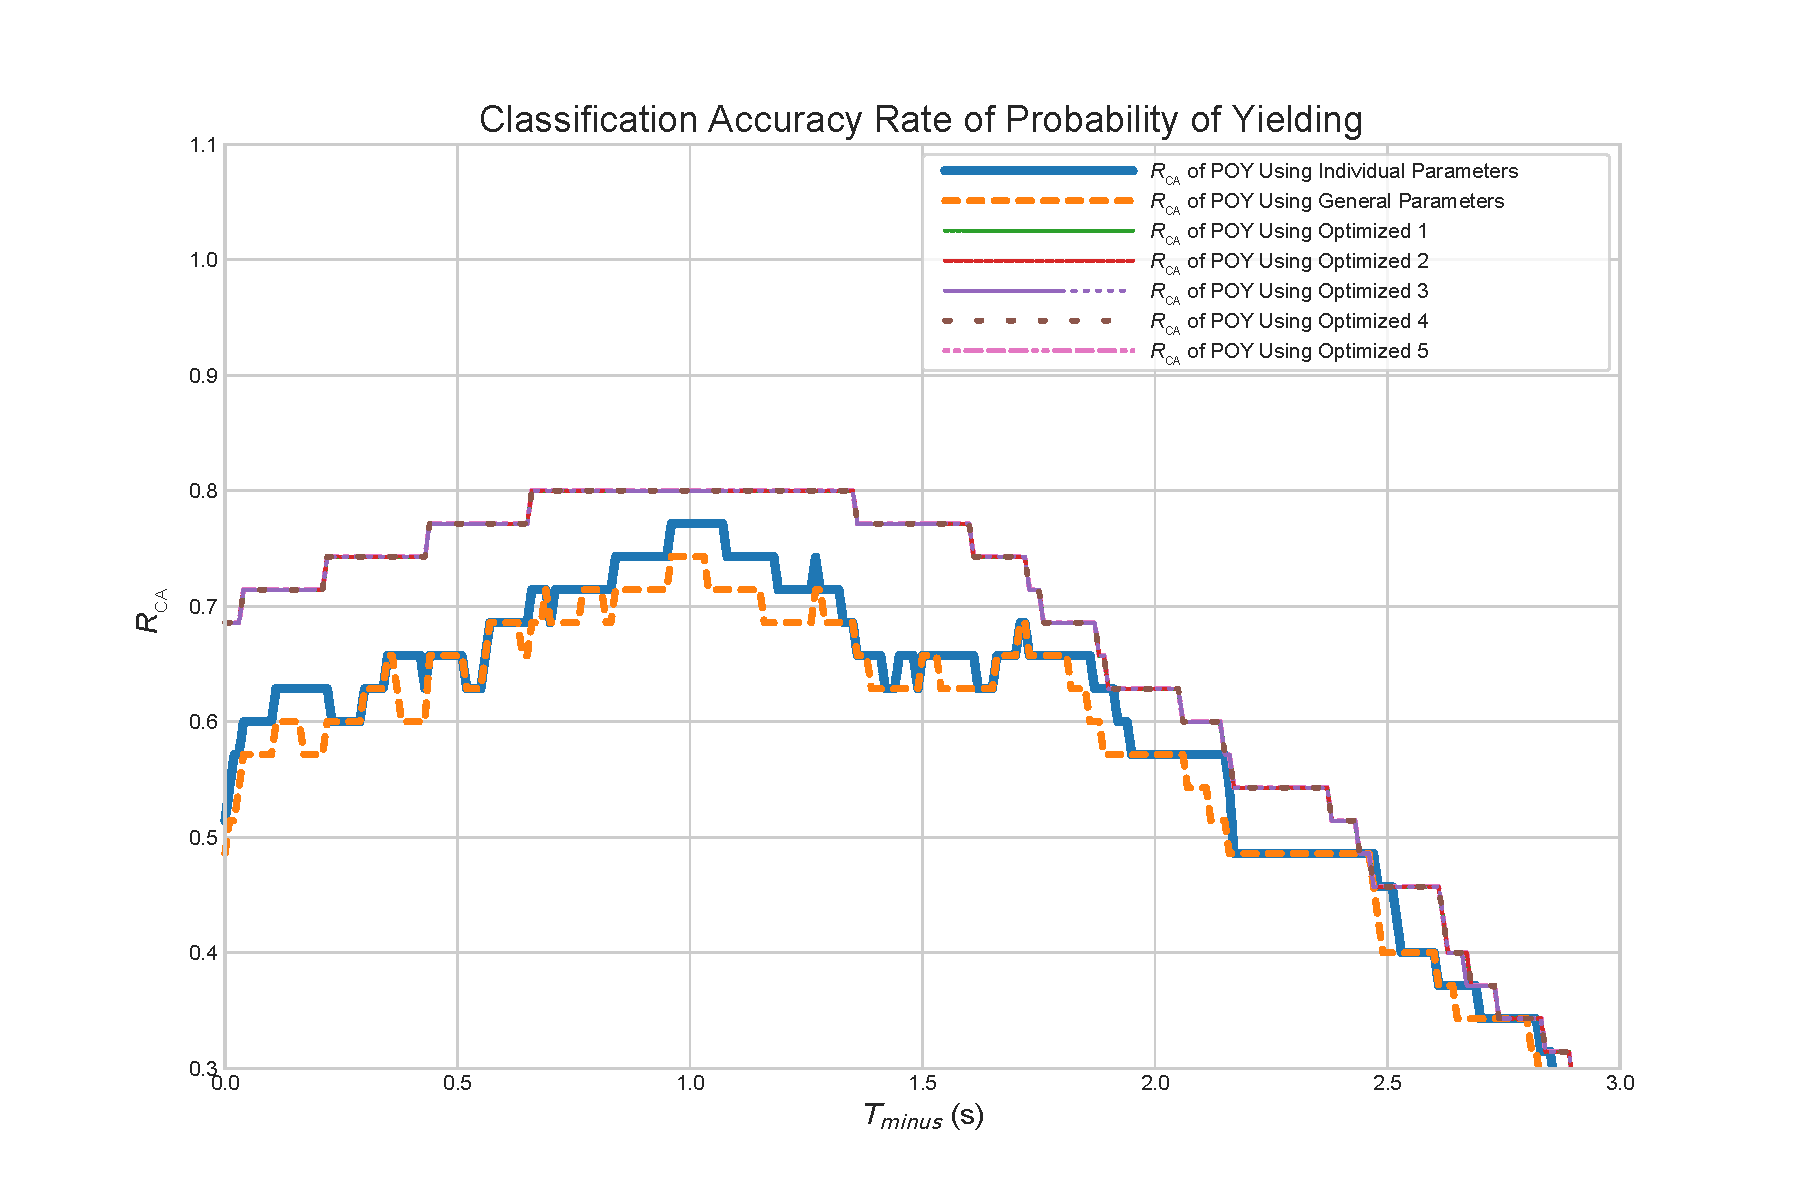
\includegraphics[width=0.64\paperwidth]{CARPOY_optimizedParam.pdf}}
\end{center}
\caption{$R_{\mathrm{CA}}$ curve of POY using characteristic parameters and optimized parameters are plotted.}
\label{fig:CAR_optimParam} 
\end{figure}

Our proposed POY model can identify possible reasons behind each crash, especially for those associated directly with driver behaviors. We are able to  evaluate the intentions of drivers at crossroads and the results are similar to those observed and verified in the simulated environment. The POY model also helps determine traffic characteristic parameters using optimization techniques. Although our results only provide a preliminary study on how to identify local traffic individuals, we show potential the practicality of the POY model in diverse extended applications. 